\documentclass[9pt]{beamer}
\usepackage{amsmath}
\usefonttheme{professionalfonts} % using non standard fonts for beamer
\usefonttheme{serif} % default family is serif\
\usepackage{mathtools}
%\documentclass[12pt]{beamerthemeSam.sty}
\usepackage{epsf}
\usepackage{ulem}
\usepackage{array}
%\usepackage{pstricks}
%\usepackage[orientation=portrait,size=A4]{beamerposter}
\geometry{paperwidth=160mm,paperheight=120mm}
%DT favorite definitions
\def\LL{\left\langle}   % left angle bracket
\def\RR{\right\rangle}  % right angle bracket
\def\LP{\left(}         % left parenthesis
\def\RP{\right)}        % right parenthesis
\def\LB{\left\{}        % left curly bracket
\def\RB{\right\}}       % right curly bracket
\def\PAR#1#2{ {{\partial #1}\over{\partial #2}} }
\def\PARTWO#1#2{ {{\partial^2 #1}\over{\partial #2}^2} }
\def\PARTWOMIX#1#2#3{ {{\partial^2 #1}\over{\partial #2 \partial #3}} }

\def\rightpartial{{\overrightarrow\partial}}
\def\leftpartial{{\overleftarrow\partial}}
\def\diffpartial{\buildrel\leftrightarrow\over\partial}

\def\BI{\begin{itemize}}
\def\EI{\end{itemize}}
\def\BE{\begin{displaymath}}
\def\EE{\end{displaymath}}
\def\BEA{\begin{eqnarray*}}
\def\EEA{\end{eqnarray*}}
\def\BNEA{\begin{eqnarray}}
\def\ENEA{\end{eqnarray}}
\def\EL{\nonumber\\}
\def\BS{\bigskip}
\def\BC{\begin{center}}
\def\EC{\end{center}}
\def\BCC{\begin{columns}}
\def\ECC{\end{columns}}
\def\HC{\column{0.5\textwidth}}
\newcommand{\etal}{{\it et al.}}
\newcommand{\gbeta}{6/g^2}
\newcommand{\la}[1]{\label{#1}}
\newcommand{\ie}{{\em i.e.\ }}
\newcommand{\eg}{{\em e.\,g.\ }}
\newcommand{\cf}{cf.\ }
\newcommand{\etc}{etc.\ }
\newcommand{\atantwo}{{\rm atan2}}
\newcommand{\Tr}{{\rm Tr}}
\newcommand{\dt}{\Delta t}
\newcommand{\op}{{\cal O}}
\newcommand{\msbar}{{\overline{\rm MS}}}
\def\chpt{\raise0.4ex\hbox{$\chi$}PT}
\def\schpt{S\raise0.4ex\hbox{$\chi$}PT}
\def\MeV{{\rm Me\!V}}
\def\GeV{{\rm Ge\!V}}

%AB: my color definitions
%\definecolor{mygarnet}{rgb}{0.445,0.184,0.215}
%\definecolor{mygold}{rgb}{0.848,0.848,0.098}
%\definecolor{myg2g}{rgb}{0.647,0.316,0.157}

\definecolor{A}{rgb}{0.8,0.0,0.0}
\definecolor{B}{rgb}{0.0,0.6,0.0}
\definecolor{C}{rgb}{0.4,0.4,0.0}
\definecolor{D}{rgb}{0.0,0.0,0.5}
\definecolor{E}{rgb}{0.4,0.4,0.4}


\definecolor{abtitlecolor}{rgb}{0.0,0.255,0.494}
\definecolor{absecondarycolor}{rgb}{0.0,0.416,0.804}
\definecolor{abprimarycolor}{rgb}{1.0,0.686,0.0}
\definecolor{Red}           {cmyk}{0,1,1,0}
\definecolor{Grey}           {cmyk}{.7,.7,.7,0}
\definecolor{Lg}           {cmyk}{.4,.4,.4,0}
\definecolor{Blue}          {cmyk}{1,1,0,0}
\definecolor{Green}         {cmyk}{1,0,1,0}
\definecolor{Brown}         {cmyk}{0,0.81,1,0.60}
\definecolor{Black}         {cmyk}{0,0,0,1}

\usetheme{Madrid}
\setbeamercolor{title}{fg=abtitlecolor}
\setbeamercolor{frametitle}{fg=abtitlecolor}
\setbeamercolor{palette tertiary}{fg=white,bg=abtitlecolor}
\setbeamercolor{palette secondary}{fg=white,bg=absecondarycolor}
\setbeamercolor{palette primary}{fg=black,bg=abprimarycolor}
\setbeamercolor{structure}{fg=abtitlecolor}

\setbeamerfont{section in toc}{series=\bfseries}

%AB: remove navigation icons
\beamertemplatenavigationsymbolsempty
\title{
  \textbf {Science and pseudoscience}\\
%\centerline{}
%\centering
%\vspace{-0.0in}
%\includegraphics[width=0.3\textwidth]{propvalues_0093.pdf}
%\vspace{-0.3in}\\
%\label{intrograph}
}

\author[W. Freeman] {Physics 211\\Syracuse University, Physics 211 Spring 2021\\Walter Freeman}

\date{\today}

\begin{document}

\frame{\titlepage}


\frame{\frametitle{\textbf{Announcements}}
\large
Recitation tomorrow will be a workshop for paper topics.

\BI
\item There will be a recitation evaluation tomorrow
\item You will have some brief homework before recitation (maybe 15-20 minutes of reading Wikipedia)
\EI
\BS
\BS\pause
We will have one more homework assignment:
\BI
\item It will be assigned Thurs/Fri and will be due next Friday
\item It will cover the physics of musical instruments
\EI
\BS
\BS
\pause
\bf There will be no recitation Friday.
}


\frame{\frametitle{\textbf{What is science?}}
	\large
	
	What is science?
	
	\BS
	
	And how is it different from other ways of gaining knowledge?
	
	\BS
	
	Tell us in Zoom or Twitch chat!
}

\frame{\frametitle{\textbf{The scientific revolution}}
	Storytime! In brief, the story of the emergence of science:
	
	\BS\BS\pause
	
	Long ago, we thought:
	\BI
	\item The Earth must be at the center of everything because we are important
	\item The stars look like they are moving so they must be
	\item Things on Earth falls because they like the ground
	\item The stars don't fall because they are heavenly
	\item Moving things come to rest on their own
	\EI
	
	\BS\BS\pause
	
	But people also figured things out:
	
	\BI
	\item The Greek/Egyptian astronomers figured out a geometric way to predict the motions of the planets
	\item The Muslim mathematicians that followed them fixed their math
	\item These calculations were very accurate
	\item ... but they were not related back to natural philosophy (the truth of nature) as a whole
	\EI
	
}

\frame{\frametitle{\textbf{The scientific revolution}}
	\large
		In the scientific revolution:
		
		\BI
		\item People made detailed {\bf observations} of the planets and did careful {\bf experiments} on moving objects
		\BS\BS
		\item People proposed {\bf models} to explain these observations
		\item They judged the validity of these models by their ability to match the data
		\item They discarded the ones that didn't work and refined ones that sort-of worked
		\BS\BS
		\item Example:
		\BI
		\item ``Maybe the planets, including Earth, go in circles around the Sun?'' -- explained retrograde motion
		\item Telescopic observations of Venus -- this {\it requires} a Sun-centered solar system
		\pause
		\item Didn't fit detailed data -- model had to be modified
		\item Circles are perfect -- but ellipses fit the data
		\EI
		\BS\BS
		
		\item Newton realized that the {\bf same set of laws} ($\vec F=m\vec a$, $F_g = \frac{GMm}{r^2}$) governed both the planets and things on Earth
		\EI
	} 

\frame{\frametitle{\textbf{Properties of science}}
	\large
	Science -- as a means of seeking truth about nature -- has a few fundamental properties:
	
	\BI
	\color{Red}
	\item {\bf Empiricism:} the ultimate authority is what we measure about the world around us, not what we think. 
	\item \normalsize The new scientific approach to mechanics started with observations: planet motion, Newton's pendulums, falling objects...
	
	\BS
	\color{Green}
	\item \large {\bf Self-skepticism:} someone making a scientific claim should actively search for things that might prove themselves wrong 
	\item \normalsize Kepler was convinced planetary orbits were circles... until the data convinced him otherwise
	
	\BS
	\color{Blue}
	\item \large {\bf Universality:} the laws of nature apply in all places and times, and to all things (including humans)
	\item \normalsize Newton was able to explain {\it all} motion with one set of principles, in space and on Earth 
	
	\BS
	\color{Brown}
	\item \large {\bf Objectivity:} scientific ideas, or the evaluation of them, should be independent of any particular human perspective
	\item \normalsize Earth was no longer given a privileged place or special rules 
	\EI
}
\frame{\frametitle{\textbf{Two notes}}

{\bf 1. ``Scientific integrity'' is not a reference to the usual sort of integrity} -- to being a good, honest person.

\BS

It is possible to do horrible things in the process of research, but do research that is well-grounded and draws correct conclusions. (Examples?)

\BS

It is also possible to be an honest, diligent scientist and make mistakes, and come to incorrect conclusions because of flaws in the application of the scientific process. (I have done this myself.)

\BS\BS

\pause

{\bf 2. There is a difference between {\color{Red}a flawed process of science} and simply being wrong.} We aren't talking 
about math errors or physics mistakes here; we're talking about {\it bypassing the safeguards in the scientific process}, either by accident or deliberately.

}




\frame{\frametitle{\textbf{Properties of science}}
\large
Broad properties of science as a means of seeking truth:

\BI
\color{Red}
\item {\bf Empiricism:} the ultimate authority is what we measure about the world around us, not what we think.
\item \normalsize It is vitally important that the conclusions we {\it claim} come from our data actually do
\item \normalsize There's a whole field of math dedicated to data analysis: {\it statistics}. It has to be done honestly and well!

\BS
\color{Green}
\item \large {\bf Self-skepticism:} someone making a scientific claim should actively search for things that might prove themselves wrong
\item \normalsize Potentially refuting arguments/evidence are a {\it good} thing

\BS
\color{Blue}
\item \large {\bf Universality:} the laws of nature apply in all places and times, and to all things (including humans)
\item \normalsize Since the laws of nature are universal, they form a coherent whole
\item \normalsize Any new finding must find its place within the framework of preexisting measurements and principles
\item \normalsize Very rarely previously-accepted things get overturned; more often they are {\it extended} 

\BS
\color{Brown}
\item \large {\bf Objectivity:} scientific ideas, or the evaluation of them, should be independent of any particular human perspective
\item \normalsize Science is not about {\it you} (whoever you are)
\item \normalsize Criticism of other people's ideas isn't about them, either 
\EI
}

\frame{\frametitle{\textbf{First, some definitions}}

\large

\BI
\item {\bf Pseudoscience:} a claim made by someone believing it is true, but that is based on deeply flawed application of the scientific process. (``They oughta know better!''). 
\pause
\BI
\item Examples: aliens making crop circles; ghosts talking through tape recorders...
\EI
\BS\BS\BS\BS\pause
\item {\bf Deliberate deception:} a claim made by someone who knows it is false, but who uses scientific language and 
trappings to lie more convincingly.
\pause
\BI
\pause
\item Examples: tobacco/cancer denialism; ``scientific racism''...
\EI
\BS\BS\BS\BS\pause
\item {\bf Honest mistakes:} a claim made by someone believing it is true, following what they believe to be sound logic, but making an honest error that leads them to a false conclusion.
\BI
\pause
\item Examples: The US Army survey of aircraft damage
\EI

\BS\BS\BS\BS

The lines between these can get kind of fuzzy...
\EI
}

\frame{\frametitle{\textbf{Common fallacies}}

\large

Let's explore some common ways that these principles get violated. This isn't an exhaustive list!

\BS\BS

Please feel free to comment in chat with your own examples. 

\BS\BS

I'd like to spend much of the time today ``off script'' -- discussing your examples, not my slides.

\BS\BS

I'll also be steering clear of any topics that are ``hot-button''. Feel free to write about these in your papers! 
But I won't be using them as examples here: the previous administration's response to COVID-19, climate change, creationism, vaccination, drug laws...
}

\frame{\frametitle{\textbf{Common fallacies: ad hominem arguments}}
\Large

{\color{Red}{\bf An ad hominem argument} is one that condemns someone else's argument because of {\it who} they are, not 
the content of their logic.}
\normalsize
\BS

\large A few types (paraphrased):

\BS
\BS


Conspiracy-type reasoning (false allegations of ulterior motives):
\BI
\normalsize
\item ``NASA faked the moon landings because they wanted to cover up the fact that their rockets didn't work''
\item ``The anti-smoking campaign is there to make money, and also something something Nazis'' (\url{http://www.smokingaloud.com})
\item ``They just {\it say} that fluoride helps dental health but it's really a Communist plot''
\EI


\BS
\BS

Arguments based on status or identity:

\BI
\normalsize
\item ``That person is an esteemed expert; we must trust them without question!''
\BI
\item Four out of five dentists recommend such-and-such brand of toothpaste...
\EI
\item ``That person is a nobody; how could they have any good ideas?''
\item ``That person is a member of race/religion/gender/political party XYZ, how could they have anything right to say?''
\EI

}


\frame{\frametitle{\textbf{Ad hominem arguments}}
\BCC
\HC
\BC
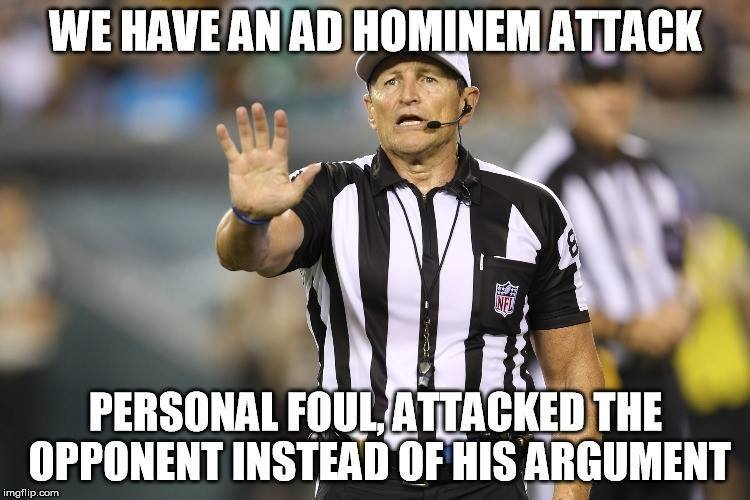
\includegraphics[width=0.8\textwidth]{ad-hom.jpg}
\EC
\HC
{\it Ad hominem} (Latin: ``against the person'') arguments fail the scientific standard of {\it objectivity}:
claims should be evaluated based on data and logic, not on who is making them.

\BS

False claims of ulterior motives are a common sort of {\it ad hominem} attack.

\ECC
\BCC
\HC

\BS\pause

... and using ``argument from authority'' is the reverse: well, if these doctors say that they smoke Camels, they must 
be safe... right?

\BS

Sometimes deliberately deceptive people really {\it do} have ulterior motives. This can be a warning sign
that someone is being deceptive...
\HC
\BC
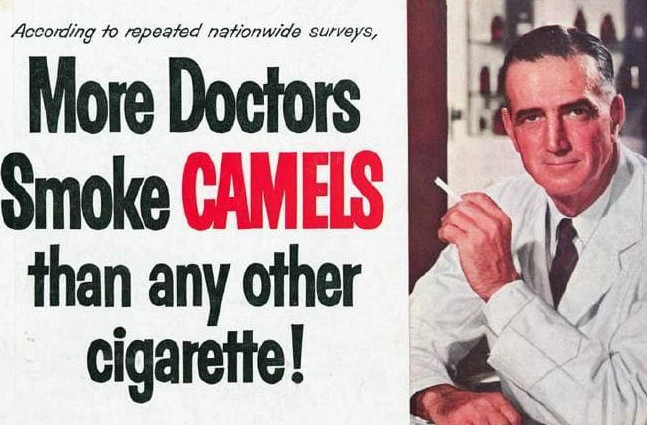
\includegraphics[width=0.8\textwidth]{tobacco-ad.jpg}
\EC
\ECC
}

\frame{\frametitle{\textbf{Ad hominem arguments}}

\Large
\BC
Do you have any favorite examples of {\it ad hominem} arguments \\being used to support flawed scientific claims?

\BS

(Comment in chat!)
\EC
\pause
\normalsize
\it\BS

``[A]fter the rocket quits our air and really starts on its longer journey, its flight would be neither accelerated nor maintained by the explosion of the charges it then might have left. To claim that it would be is to deny a fundamental law of dynamics, and only Dr. Einstein and his chosen dozen, so few and fit, are licensed to do that....
That Professor Goddard, with his ``chair" in Clark College and the countenancing of the Smithsonian Institution, does not know the relation of action and reaction [Newton's third law], and of the need to have something better than a vacuum against which to [push] -- to say that would be absurd. Of course he only seems to lack the knowledge ladled out daily in high schools.''

\BS
\rm
\begin{flushright} --\it The New York Times\rm, 1920\end{flushright}

\pause
\BS\BS\BS


``\it Further investigation and experimentation have confirmed the findings of Isaac Newton in the 17th Century and it is now definitely established that a rocket can function in a vacuum as well as in an atmosphere. The \rm Times \it regrets the error.''

\BS
\rm
\begin{flushright} --\it The New York Times\rm, 1969 \end{flushright}
}

\frame{\frametitle{\textbf{Statistical dishonesty}}
\large
{\color{Red}Statistics} is the mathematical discipline that lets us turn empirical data into conclusions.

\BS

It lets us turn a collection of ``maybes'' and ``probablys'' and ``unlikelys'' into ``almost certainlys''.

\BS\BS

\normalsize

Statistics is immensely powerful. But:

\BI
\item It is a subtle, complex field of math (you can get PhD's in it)
\item It is a lot of work and only someone intimately familiar with data is really equipped to analyze it
\pause
\item {\color{Red}It is absolutely essential if science is going to look to empirical data as the highest authority}
\EI

\BS
\BS

A great many flawed scientific processes come down to flawed statistics. Some common statistical fallacies:

\normalsize
\BI
\item ``Garbage in, garbage out'': flawed, stinky data $\rightarrow$ statistical analysis $\rightarrow$ incorrect but nonstinky conclusions!
\item Correlation implies causation: does the decline in pirates cause climate change?
\item Incorrect use of statistical inference (statistics is hard)
{\color{Red}
\item Some types of statistical shenanigans (often related to sampling bias):
\BI
\item ``P-hacking''
\item Publication bias
\EI
}
\EI
}

\frame{\frametitle{\textbf{Statistical inference done honestly}}

Suppose we want to test if a new drug (or a chemical in food) has any effect.

\BS

Correct thing to do:

\BI
\item Make lots of measurements of how people react to the drug
\item Compare their distribution to the black curve (what you'd expect if the drug does nothing)
\item Get excited if their average is very different from the center of the curve (maybe drug made that happen?)
\BI
\item (Statistics gives us tools to quantify ``very different'')
\EI
\EI


\BC
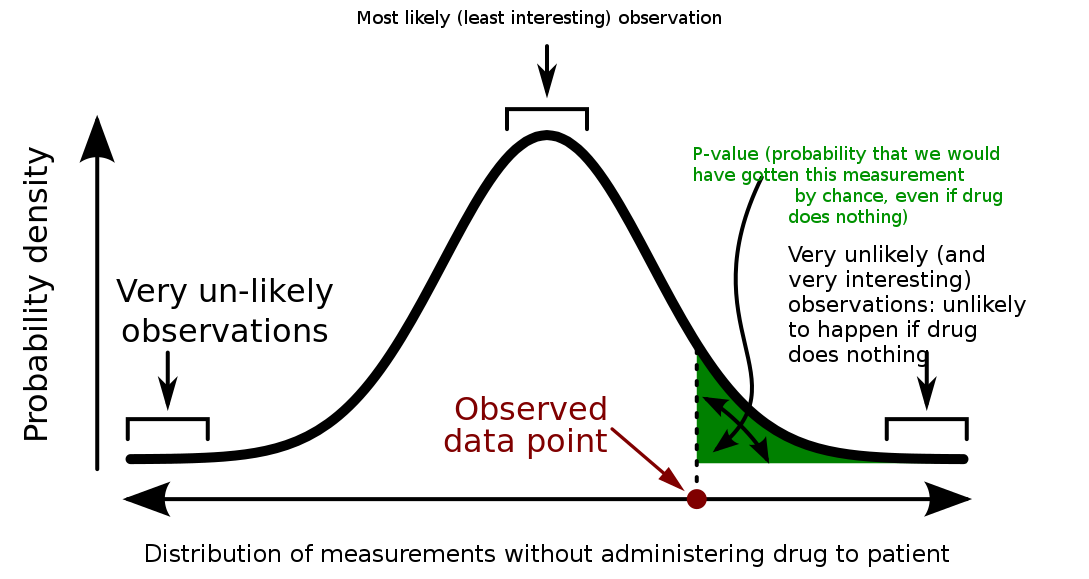
\includegraphics[width=0.8\textwidth]{gaussian.png}
\EC
}

\frame{\frametitle{\textbf{Statistical inference gone wrong, I: cherry-picking}}

\BS

Classic cherry-picking:
\BI
\item Make lots of measurements of how people react to the drug
\item {\color{Red} Forget about the ones close to the center (they are boring!)}
\item Compare their distribution to the black curve (what you'd expect if the drug does nothing)
\item {\color{Red} Even if the drug does nothing, you'll get a distribution looking like the green portion}
\item {\color{Red} Notice that their average is very different, get excited!}
\EI


\BC
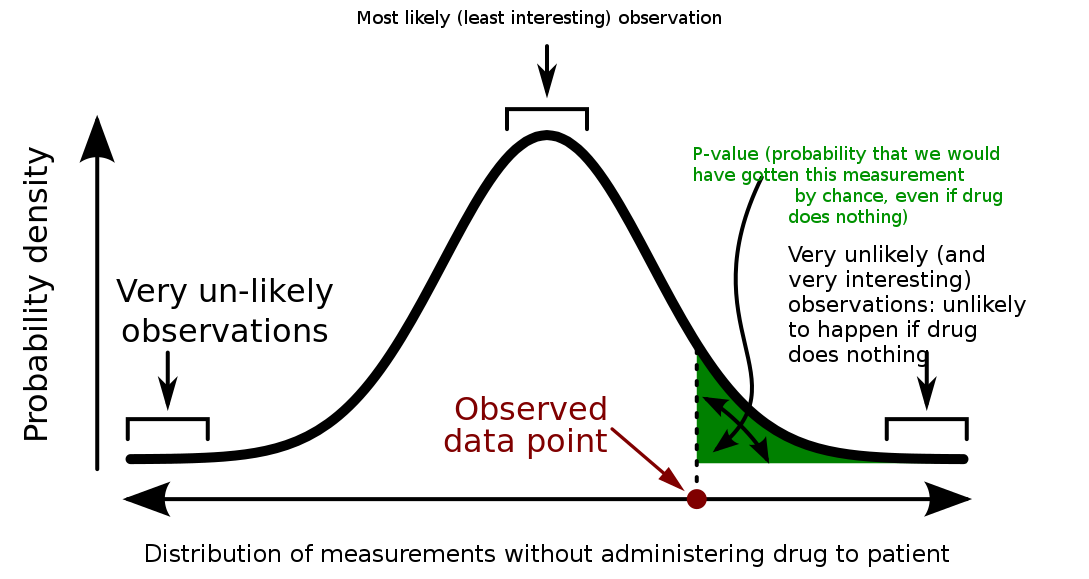
\includegraphics[width=0.8\textwidth]{gaussian.png}
\EC
}

\frame{\frametitle{\textbf{Statistical inference gone wrong, II: biased data}}

\BS

One example of biased data is {\it survivorship bias:}
\BI
\item Make lots of measurements of how people react to the drug
\item {\color{Red} Fail to measure the ones on the left-hand side (they're dead)}
\item Compare their distribution to the black curve (what you'd expect if the drug does nothing)
\item {\color{Red} We removed the left-hand side, so the average shifts right}
\item {\color{Red} Notice that their average is very different, get excited!}
\EI

\BC
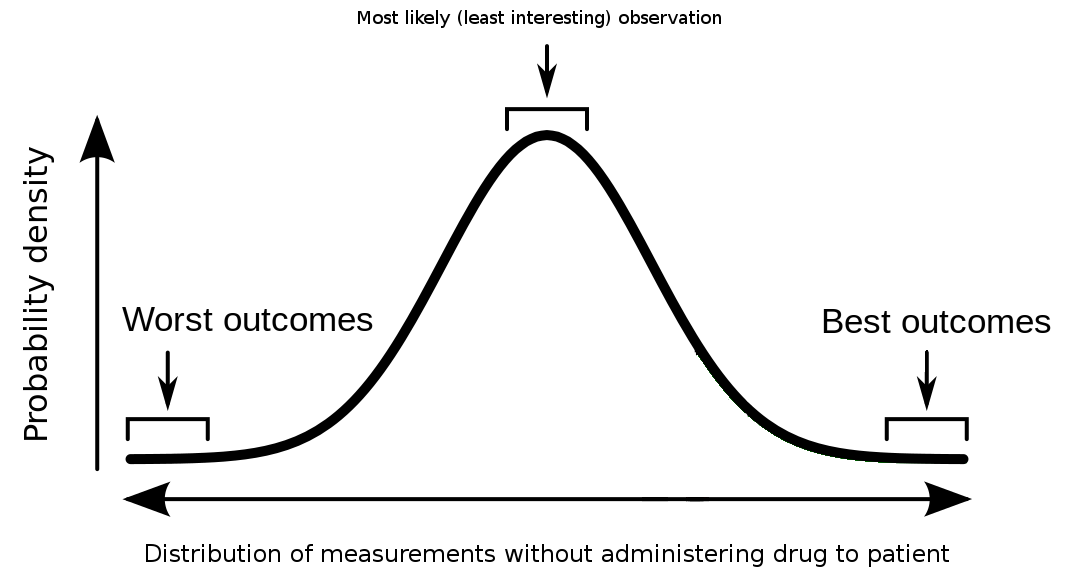
\includegraphics[width=0.8\textwidth]{gaussian2.png}

\BS
\pause
{\color{Green}This sort of thing happened in a hydroxychloroquine study in 2020!}
\EC
}

\frame{\frametitle{\textbf{Statistical inference gone wrong, III: publication bias}}

\BS

If the measurements are entire {\it studies}, we often unintentionally cherry-pick them in {\it meta-analyses} (studies 
averaging many studies together)
\BI
\item Different scientists do experiments on how people react to the drug
\item {\color{Red} Nobody publishes the ones close to the center (they're boring, back to the drawing board!) }
\item Compare their distribution to the black curve (what you'd expect if the drug does nothing)
\item {\color{Red} Even if the drug does nothing, you'll get a distribution looking like the green portion}
\item {\color{Red} Notice that their average is very different, get excited!}
\EI


\BC
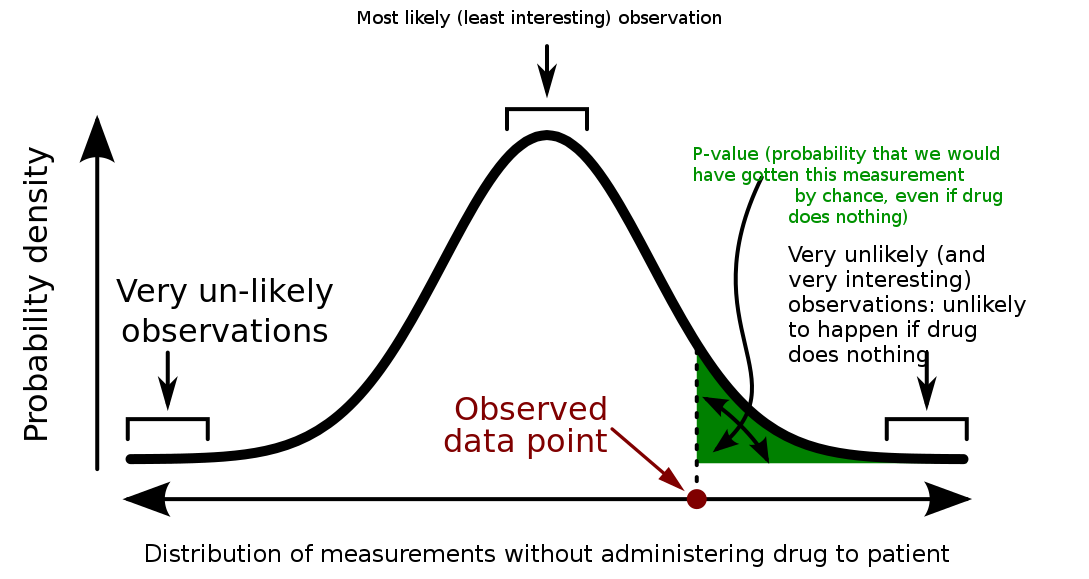
\includegraphics[width=0.8\textwidth]{gaussian.png}
\EC
}

\frame{

\large
\BC
Do you have any favorite examples of statistical shenanigans being used to support flawed claims?

\BS

(Discuss them in chat)
\large
\EC

\BS\pause
\BS
The above example about drug studies is real: publication bias is a serious problem in drug 
development! (See \url{https://www.nejm.org/doi/full/10.1056/NEJMsa065779})
\vfill

}


\frame{\frametitle{\textbf{Ignoring refuting evidence}}

\BS

\begin{columns}
\column{0.6\textwidth}
{\color{Green} Self-skepticism} is a hallmark of sound science. Good scientists report:
\small
\BI
\item Any experimental evidence that might conflict with their proposal
\item All of the possible flaws that {\it they} thought of in their claim
\BI
\item ... and how they considered them
\EI
\item Any tests that anyone {\it else} could do to try to disprove them
\item All the things that make them {\color{Red} uncertain} about their result
\item The limits of their conclusions
\EI
\column{0.4\textwidth}
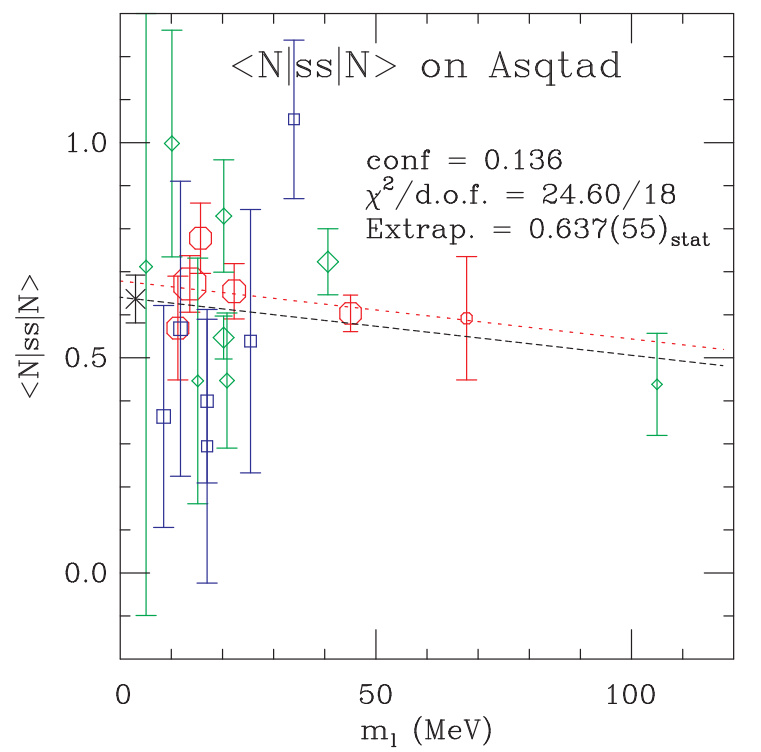
\includegraphics[width=\textwidth]{extrap.jpg}
\scriptsize \it A figure from my PhD thesis. I spent probably five times as much effort on quantifying the uncertainty in my results than I did getting the result itself. All the complicated statistics above was in service of this!
\ECC
\BS\BS

Most good scientific writing spends much of its time doing the above. You should only try to convince
other people you are right once you have 
tried very hard, yet failed, to prove yourself wrong.

\BS

\BC\color{Red}Any claimant that spends most of their time talking {\it up} their conclusions is likely suspect.\EC

}

\frame{\frametitle{\textbf{Ignoring potentially refuting evidence}}
\large

{\color{Red}Ignoring or failing to search for refuting evidence} is a common trait of faulty scientific process. 
This can either be:

\BS
\BI
\item Ignoring refuting evidence altogether, even if it's widely known
\item Dismissing refuting evidence out of hand, without considering it in any real way 
\item Failing to think of potentially refuting evidence and search for it
\EI
\Large
\BC

\BS\BS\BS

Do you have any favorite examples of flawed scientific claims \\that fail to address potentially refuting evidence?

\BS

(Discuss them in chat!)
\large
\EC

\large

\BS
\BS\BS\BS
\BC
\url{https://wiki.tfes.org/Flat_Earth_-_Frequently_Asked_Questions}
\EC

}

\frame{\frametitle{\textbf{Ignoring the rest of science: ``island claims''}}
\Large
Natural laws are {\color{Red} universal}: the laws of physics are the same everywhere and at all times.

\BS

\normalsize

This means that a new idea doesn't just have to fit together with the evidence used to support it, and a few bits 
of potentially refuting evidence.

\BS

It has to play nice with {\bf all} other data, from centuries of experience. 

\BS

If you're proposing a new fundamental law of physics, it has to be compatible with {\it everything} else.

\BS

\pause

\BI
\item We see nuclear reactions that don't seem to conserve momentum; what happened?
\pause
\item {\color{Red} ... there's another particle produced we can't detect (the neutrino)}

\BS\BS\BS

\item The following things are mutually inconsistent; what do we do?
\BI
\item Electromagnetism (very well tested in the lab)
\item The independence of space and time (seems obvious to everyone, right?)
\item A universe that fundamentally makes sense (we all agree on how things will happen, etc.)
\EI
\item {\color{Red} ... turns out space and time {\it aren't} independent} -- this sort of revolution is rare!
\EI
}

\frame{\frametitle{\textbf{Ignoring the rest of science: ``island claims''}}
\Large
If you're proposing a new machine, then there needs to be a plausible explanation for how it works.

\BCC
\HC
\BC
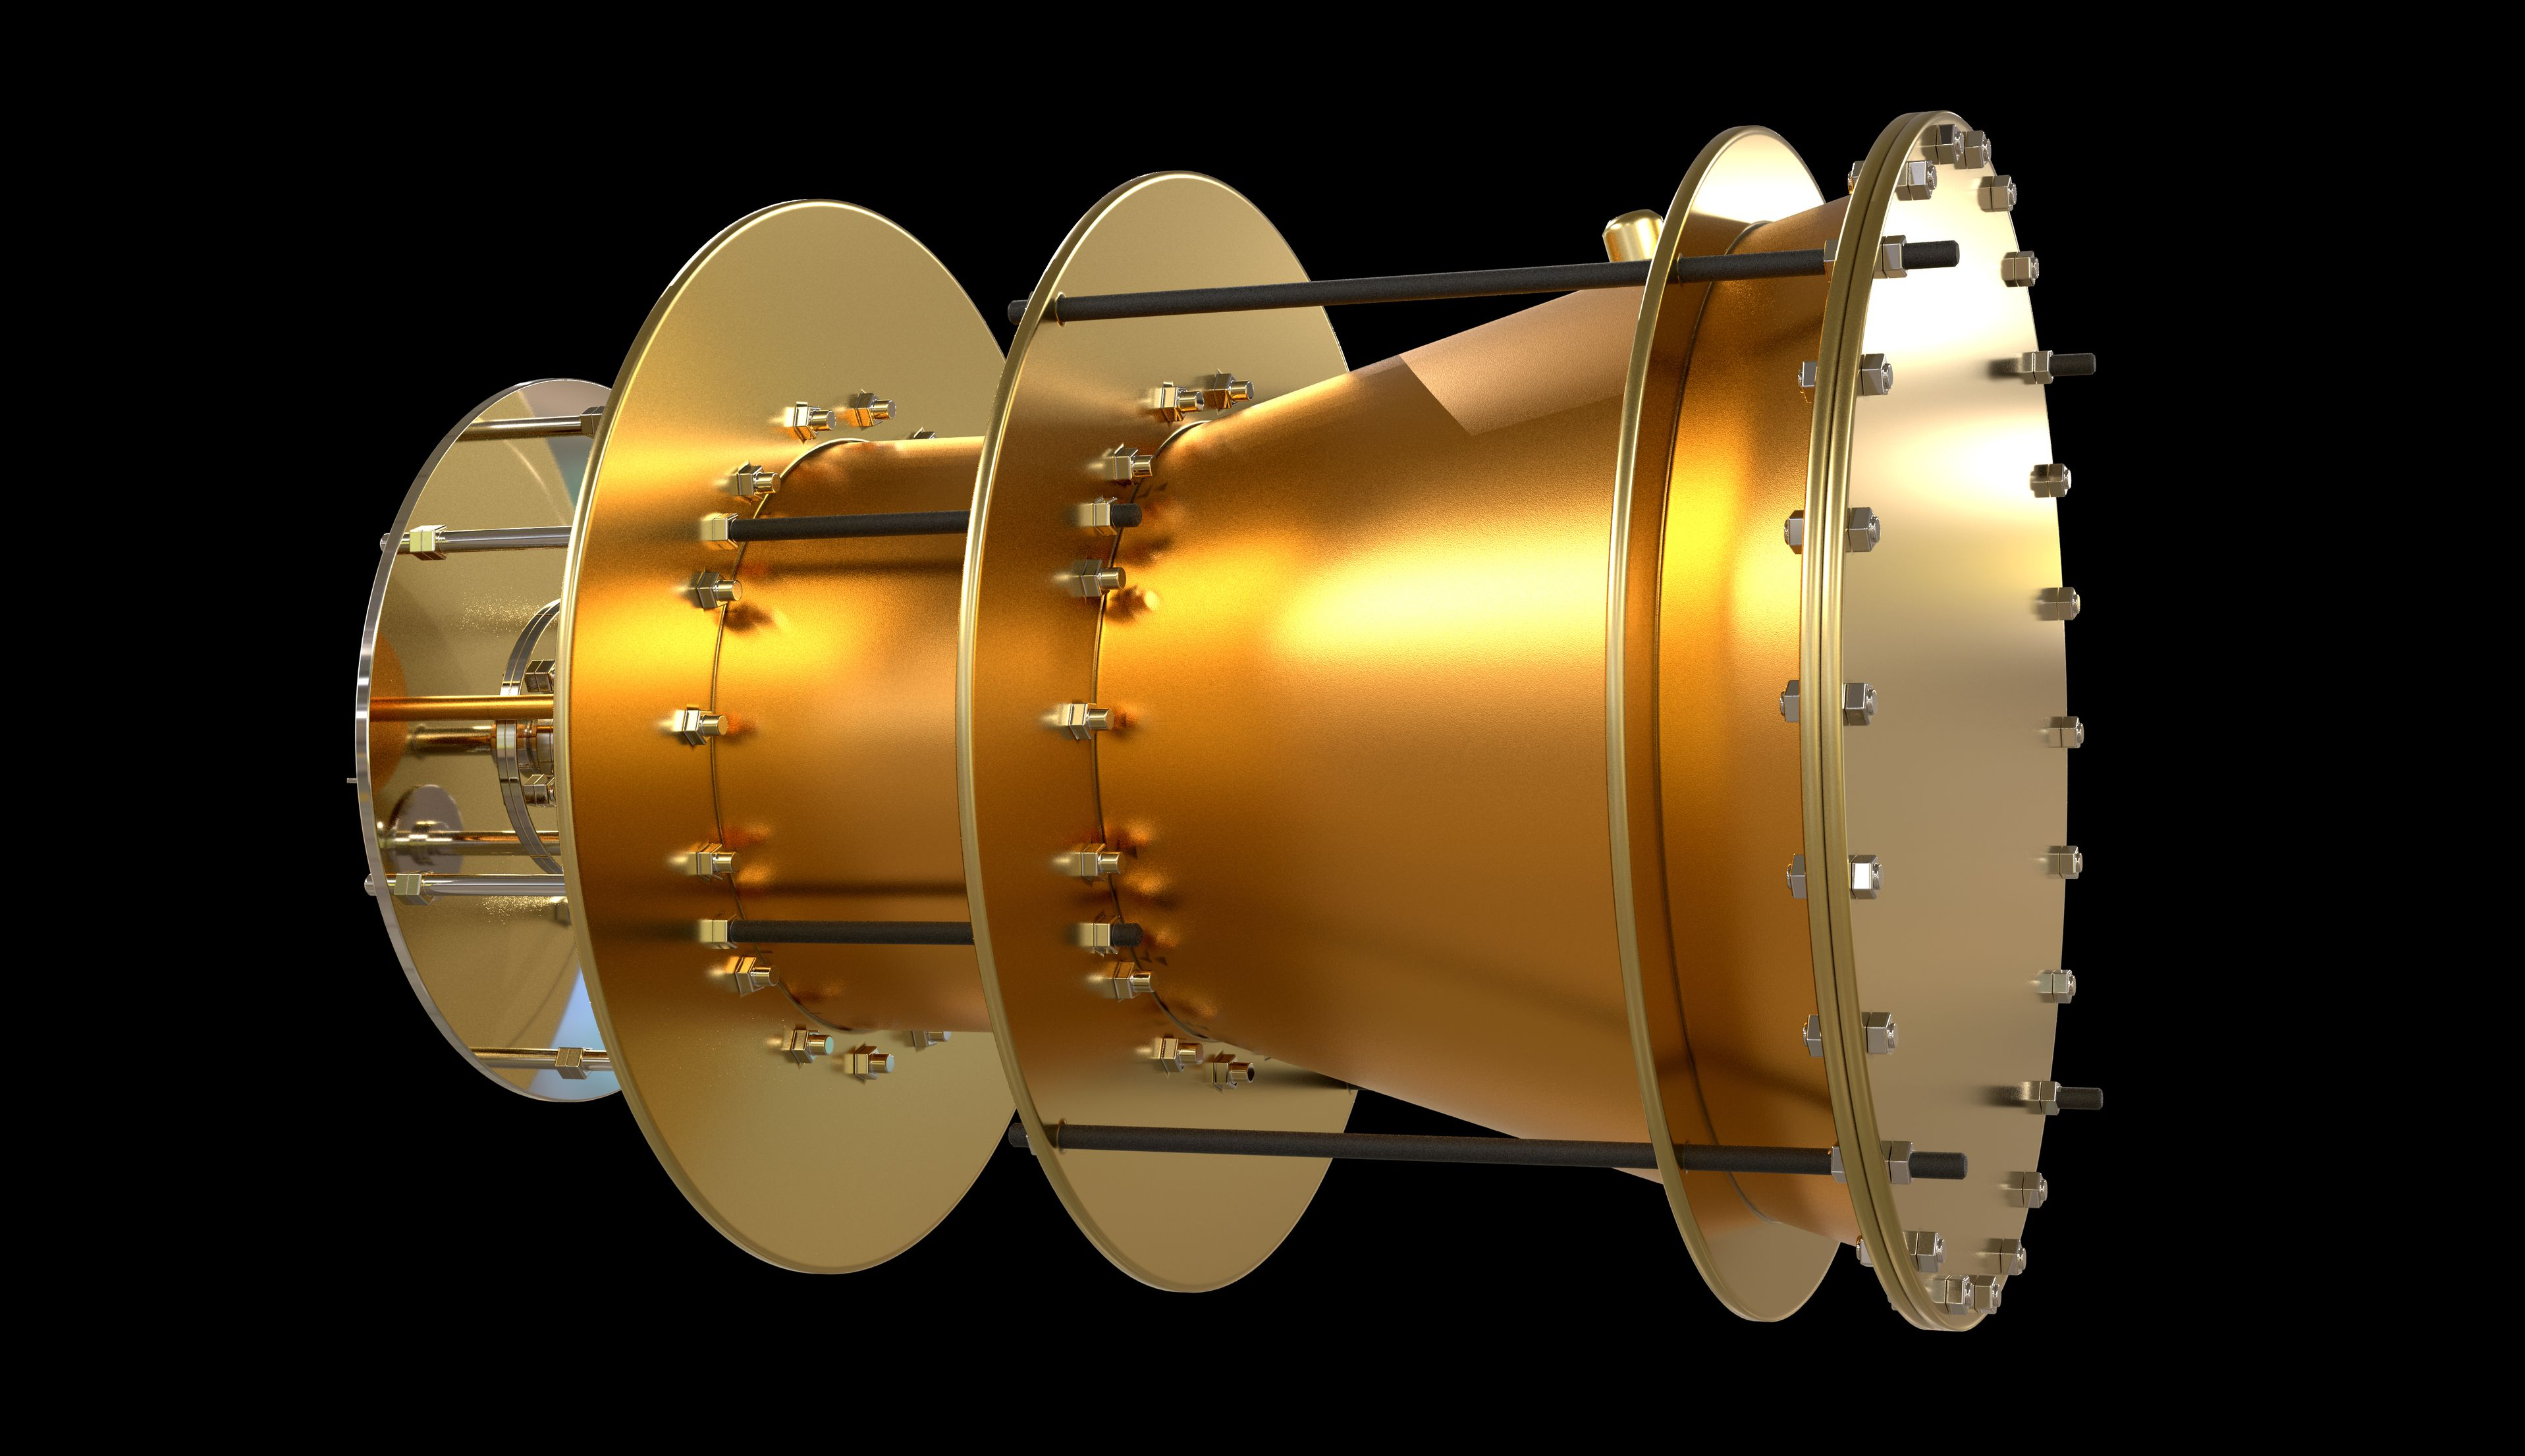
\includegraphics[width=0.85\textwidth]{emdrive.jpg}

\small \it ``The EM-Drive'', not actually a rocket engine
\EC
\HC
\large
People claimed this is a rocket motor that uses no fuel (reaction mass), only an energy source.

\BS

They acknowledged that it seemed to violate Newton's third law / the conservation of momentum, but 
had no explanation for how it actually {\it did} work. But they claimed it produced a tiny fraction of a 
newton of thrust.

\ECC
\BS
\BS
\BC
(It didn't. It was interference between the machine and the measuring equipment. It's hard to measure 
a tiny force on a huge thing in the context of lots of microwaves.)
\EC
}


\frame{\frametitle{\textbf{Manufacturing a controversy}}
\large
We've discussed some of the common features of people {\it advancing scientific claims}
incorrectly, negligently, or dishonestly.

\BS
\BS

Sometimes dishonest people aren't trying to {\it advance} something they know to be false, though.

\BS

They're more interested in convincing people to {\it reject} something that is true.

\BS

To do that, they only need to create doubt. This is commonly done by {\it manufacturing a controversy}.

\BS\pause

\BS\BS
\normalsize

(This is a common tactic to erode trust in {\it anything}, not just science -- common in politics and negative advertising)
}

\frame{\frametitle{\textbf{Manufacturing a controversy}}

\Large
\BC
Do you have any favorite examples of manufactured controversies?
\EC

\pause

Consider again the tobacco industry:

\BI
\item ``Secondhand smoke doesn't cause health problems; those studies are wrong''
\item ``Are you really sure that secondhand smoke causes health problems? Maybe it was poor building ventilation!''
\EI

One of these is a far easier sell than the other!

\BS
\BS
\normalsize
{\it The industry's strategy does not require winning the debates it manufactures. It is enough to foster and perpetuate the illusion of controversy in order to muddy the waters around scientific findings that threaten the industry. Thus it offers reassurance to smokers, helping them to rationalize and repress their health concerns. Furthermore, claims of ``not proven'' resonate with friendly or naive journalists and governments, and provide an excuse for not taking strong governmental or societal action against tobacco.}

\scriptsize
\BS
\begin{flushright}--Yussuf Saloojee and Elif Dagli,  "Tobacco industry tactics for resisting public policy on health" Bull. World Health Organ. 78(7): Genebra, July 2000.\end{flushright}
}



\frame{\frametitle{\textbf{Sensationalism}}
\Large
Two things are both true:

\BI
\item Some scientific findings can dramatically change our lives and our perspective on the world, and are compelling and exciting
\item Whether a scientific claim is true or not doesn't depend on whether it's exciting or not (objectivity)
\EI

\BS\BS

Scientists thus have twin duties:

\BI
\item They should engage with society in sharing the excitement and interest of their findings. Science communication is vital (and many of us are bad at it; the astronomers do better than the physicists!)
\item They should {\color{Red} separate this excitement} from the task of {\color{Green} evaluating the validity of claims}
\EI
}

\frame{\frametitle{\textbf{Sensationalism}}
\large
Beware of any sort of scientific claim that conflates {\color{Red}the evidence that it is true} with {\color{Green}why you should be excited by it}, or that seems to be {\color{Blue}hyped by its claimant}.

\BS
\BS

Good scientists do hold press conferences, because many discoveries are exciting!

\BS

But these happen only in the context of:

\BI
\item a vast amount of self-skepticism applied to their results first
\item objective, sober presentation of the {\it evidence} for their conclusions, not just why they are exciting
\EI

\BS
\BS
}

\frame{\frametitle{\textbf{Sensationalism}}
	\BC
	Do you have any favorite examples of over-sensationalized scientific claims?
	\EC

}
%
%\frame{\frametitle{\textbf{Black holes}}
%Now -- what about black holes, and pictures of them from Earth?
%
%\url{https://iopscience.iop.org/journal/2041-8205/page/Focus_on_EHT}
%
%\url{https://arxiv.org/abs/1802.05783}
%
%}
%
%
%\frame{\frametitle{\textbf{Black holes}}
%	
%	A black hole is a place where matter is so dense that its gravity becomes strong enough that light can't escape.
%	
%	\BS
%	
%	The black hole is surrounded by a boundary called the {\it event horizon}, which delinates the region from which light can't escape.
%	
%	\BS
%	
%	Anything that gets near a black hole orbits it, like the planets orbit the Sun. But:
%	
%	\BI
%	\item Friction between these bits of dust does negative work on them, reducing their velocity
%	\item This reduces their kinetic energy, so gravity pulls them closer to the black hole
%	\item This does positive work on them (practice exam question!), speeding them back up. 
%	\item As they get closer and closer, they get hotter and hotter, and glow brighter and brighter
%	\EI
%	
%	The event horizon can be surrounded by a glowing disk of gas at millions of degrees.
%	
%	\BCC
%	\HC
%	\BC
%	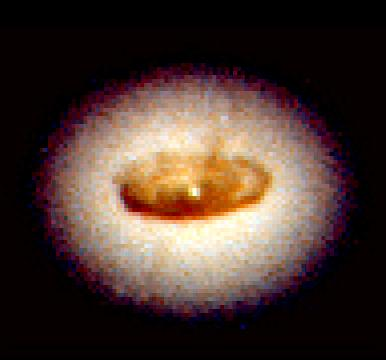
\includegraphics[width=.5\textwidth]{bh-hubble.jpg}\\
%	\it\scriptsize (Hubble image of a very bright accretion disk)
%	\EC
%	\HC
%	\BC
%	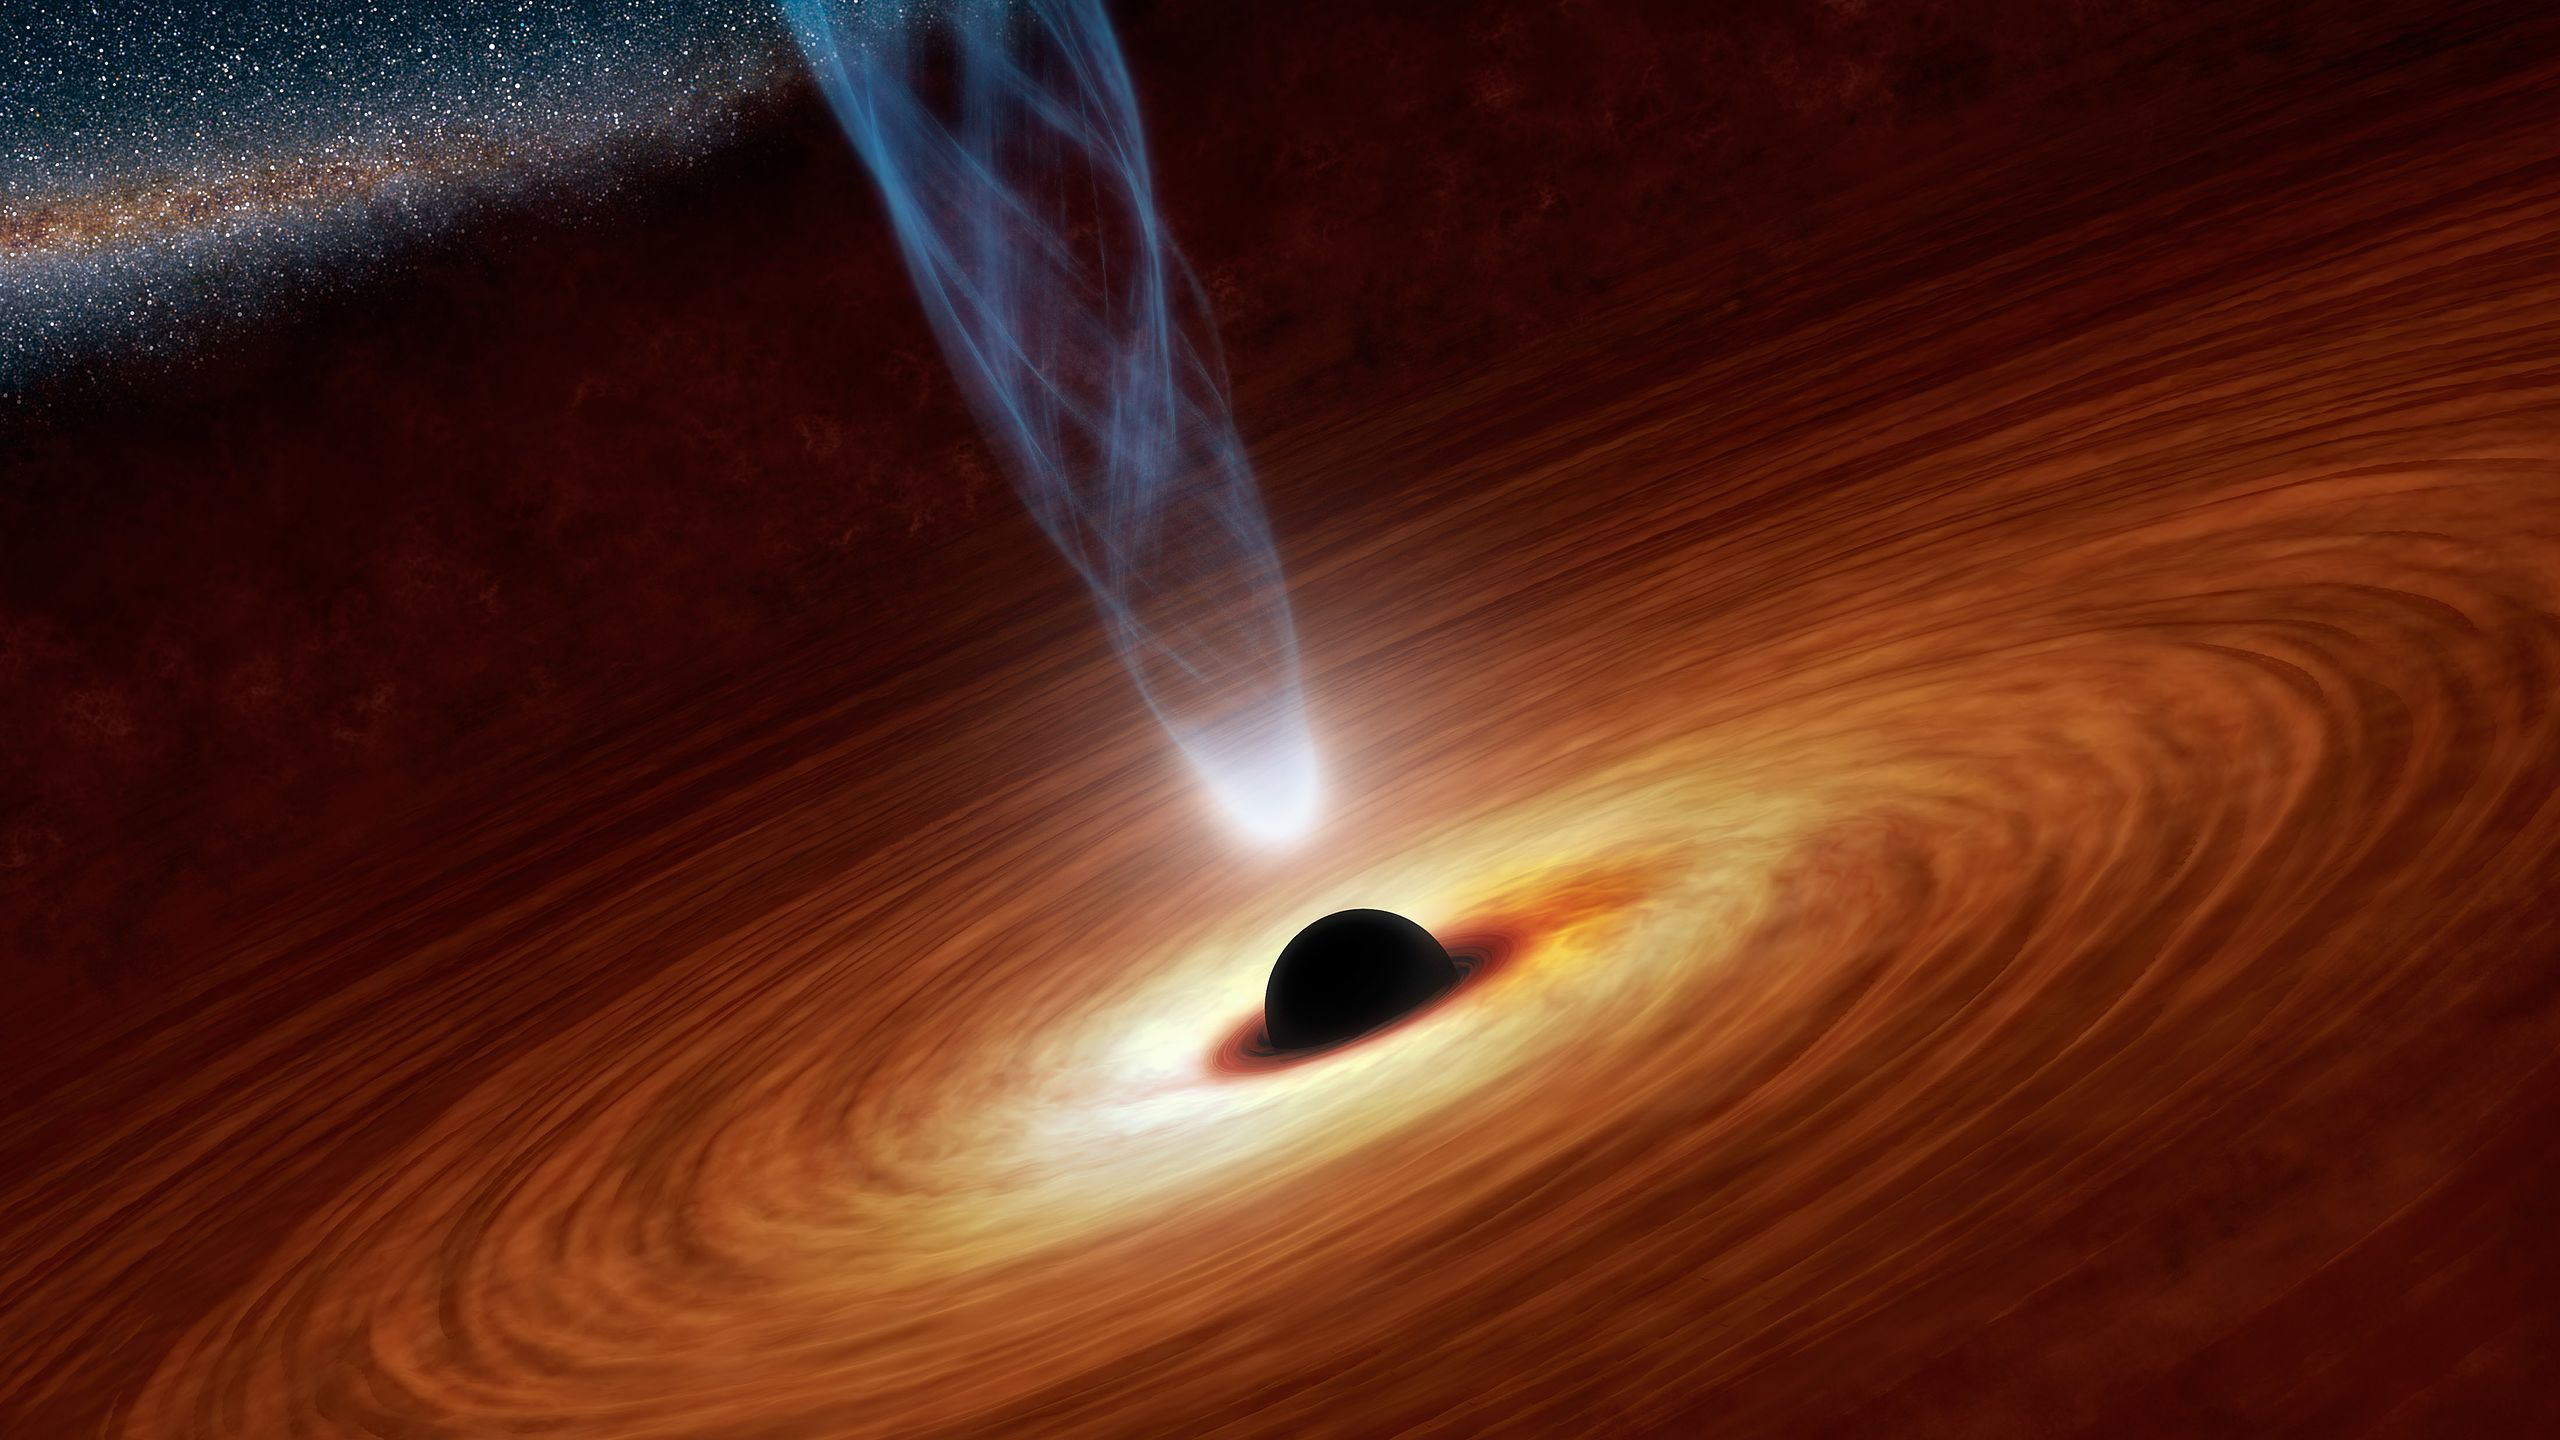
\includegraphics[width=.8\textwidth]{bh-render.jpg}\\
%	\it\scriptsize (Artist's rendering, if the BH didn't bend its own light)
%	\EC
%	\ECC
%}
%
%
%
%\frame{\frametitle{\textbf{Black holes}}
%	
%	\large
%	
%	There are two types of black holes:
%	
%	\BI
%	\item Ones that form from the dead cores of huge stars (mass of a few times that of our Sun)
%	\item Ones that form from the junk that falls to the center of a galaxy (mass billions of times larger)
%	\EI
%	
%	This recent image is of a supermassive black hole around 50 million light years away, at the core of 
%	a galaxy called M87.
%	
%	\BS\BS
%	
%	This is exciting because it's an image of the {\it actual event horizon}, not just the {\it accretion disk}.
%}
%
%\frame{\frametitle{\textbf{Interferometry}}
%	
%	\large
%	
%	The smallest angular size you can make out in a picture is given by:
%	
%	$$\theta = \frac{\text{wavelength of light}}{\text{(size of lens)}} $$
%	
%	So, to get a detailed picture, you need to measure very short wavelengths with a very big aperture (lens/mirror size).
%	
%	\BS\BS
%	
%	Your ``aperture'' is just the region over which you can correlate the {\it phase} (whether a wave is going up or down at any given time)
%	at different points. 
%	
%	\BS
%	
%	If you can do that by another means (by making a machine that detects phase as well as the presence of light), you can count different observing stations as part of the same
%	aperture.
%	
%	\BS
%	
%	This process is called ``interferometry'' or ``synthetic aperture imaging''.
%}
%
%\frame{\frametitle{\textbf{Two ways to make a big eyeball}}}
%
%\frame{\frametitle{\textbf{Interferometry}}
%	
%	\BCC
%	\HC
%	\BS
%	
%	This gets harder as the frequency goes up, since the wave switches from ``up'' to ``down'' faster.
%	
%	\BS
%	
%	Also: frequency is inversely proportional to wavelength.
%	
%	\BS
%	
%	Remember that we need a combination of {\it large aperture} and {\it short wavelength} (meaning high frequency) to
%	get a detailed picture.
%	\HC
%	
%	\BC
%	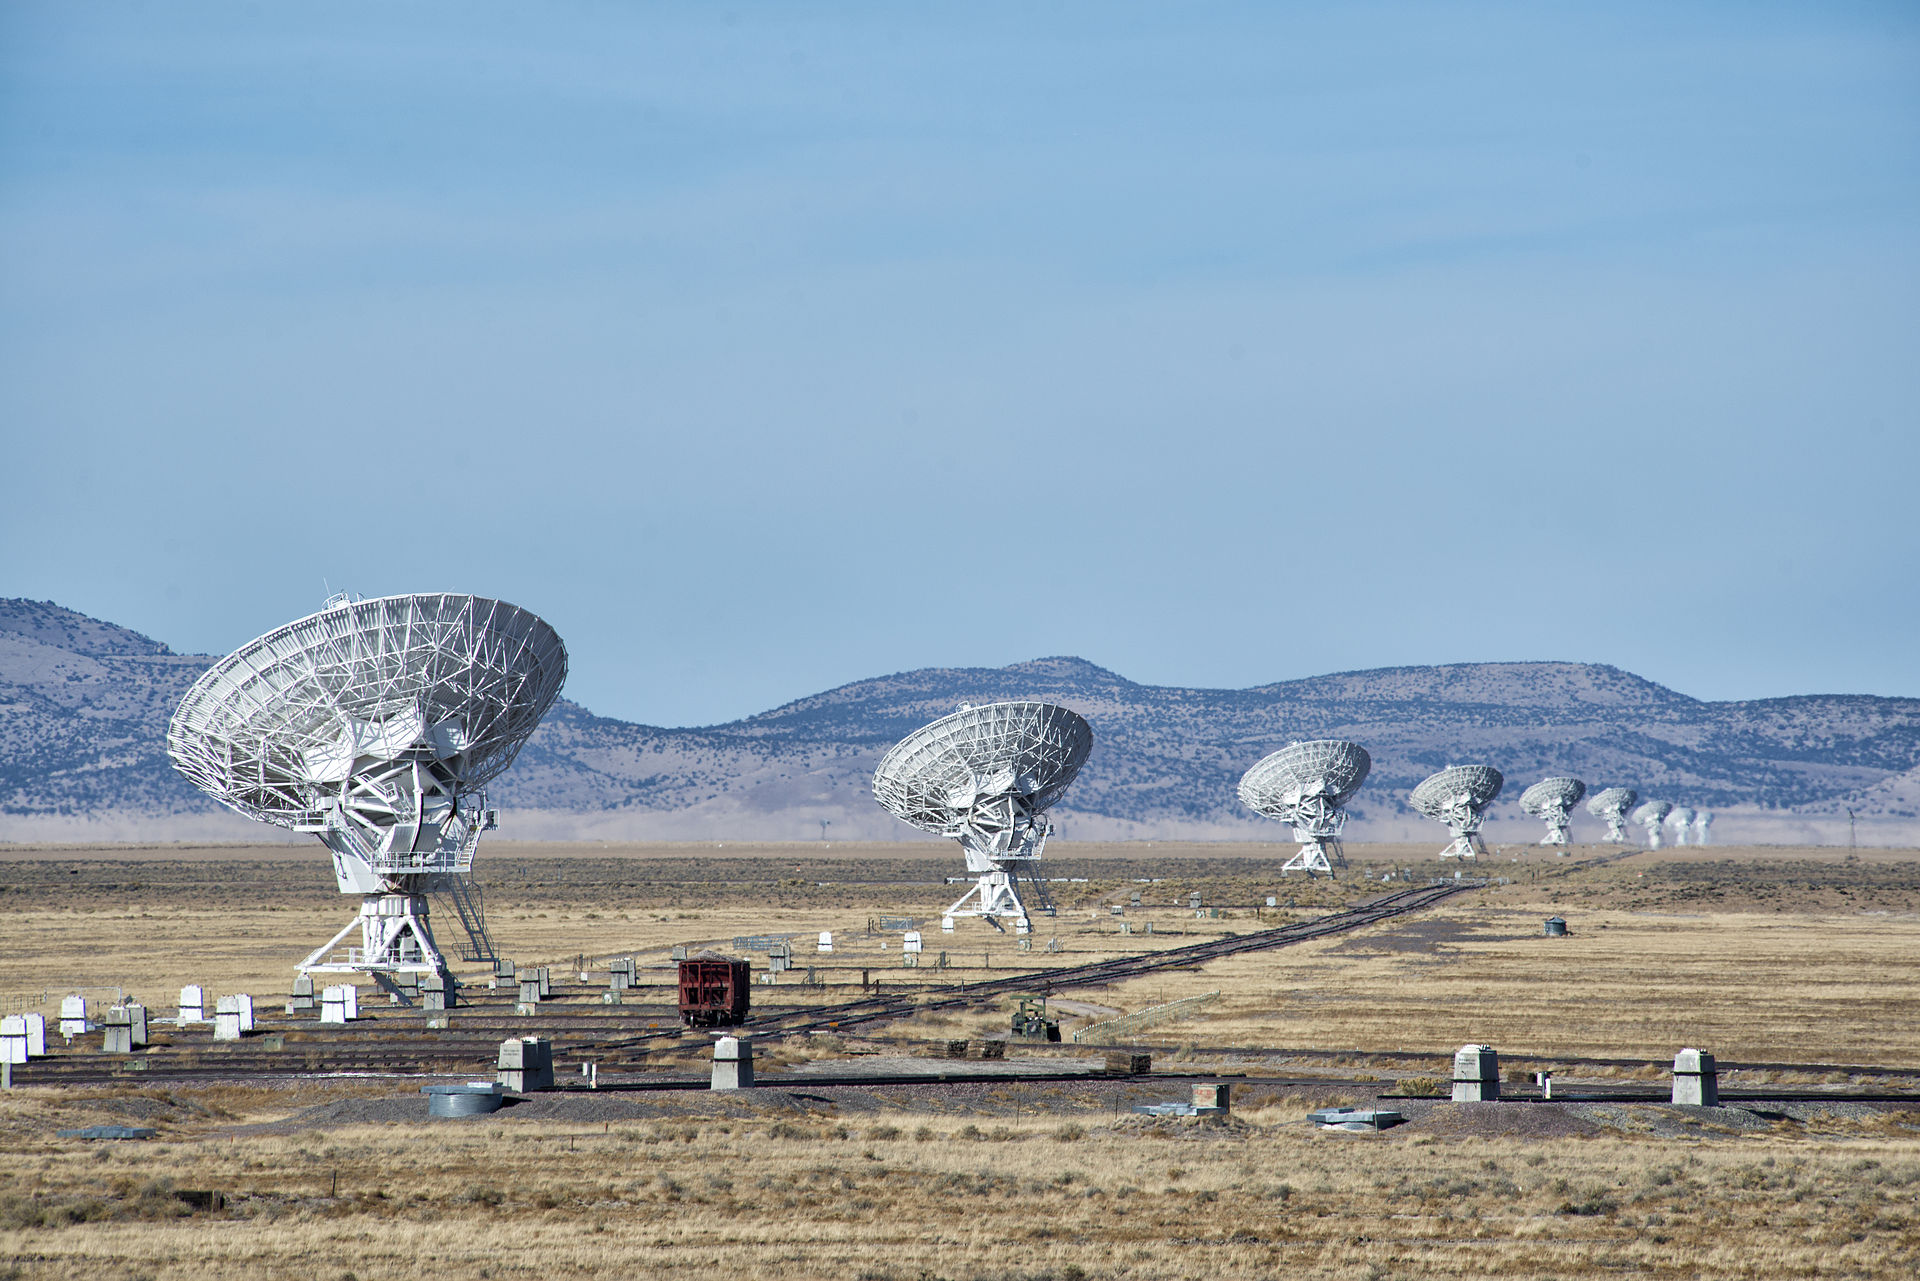
\includegraphics[width=0.9\textwidth]{vla.jpg}\\
%	\it \scriptsize The Very Large Array, a synthetic aperture radio ``telescope'', in New Mexico. The telescopes 
%	are on railroad tracks to allow operators to customize the aperture shape.\EC
%	\ECC
%	\BS\BS
%	
%	The problem:
%	
%	\BI
%	\item The very shortest wavelengths (x-rays, $\gamma$-rays) don't bend in lenses or bounce off mirrors well
%	\item Mid-range wavelengths (like light) are long enough that it's hard to make a clear picture without a physically
%	huge aperture, but have frequencies too fast to do interferometry
%	\item Radio waves have a slow enough frequency to do interferometry, but have too long of a wavelength to get a clear
%	picture even with an enormous synthetic aperture
%	\EI
%}
%
%\frame{\frametitle{\textbf{The Event Horizon Telescope}}
%	
%	The solution, allowing the Event Horizon Telescope to observe extremely fine detail:
%	
%	(Remember: we want a large aperture and short wavelength/high frequency)
%	
%	\BCC
%	\HC
%	\BI
%	\item Combine data from radio telescopes across the hemisphere
%	\item This gives an enormous synthetic aperture (diameter the size of Earth)
%	\item Develop very accurate ways to measure and correlate phase over long distances (timing equipment)
%	\item Measure at very high frequencies (a few thousand times FM radio)
%	\item {\color{Red} You now have a radio telescope the size of Earth, measuring very short wavelengths}
%	\EI
%	\HC
%	\BC
%	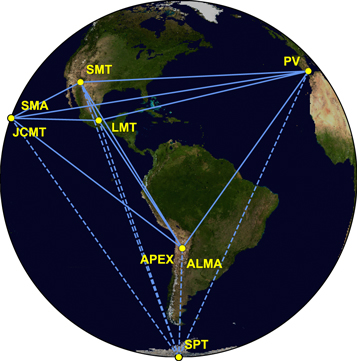
\includegraphics[width=0.9\textwidth]{eht.jpg}\EC
%	\ECC
%}
%
%\frame{\frametitle{\textbf{The Event Horizon Telescope}}
%	Since this is a synthetic aperture, doing the data processing is hard.
%	
%	\BS
%	
%	Imagine using a camera with the whole lens blacked out, except for a few tiny pinholes, and that's constantly spinning!
%	
%	\BS
%	
%	Some very clever folks had to develop new math and algorithms for image analysis and reconstruction to do this (Katie Bouman did this, and also became famous for her communication work on this project)... but here's the result:
%	
%	\BC
%	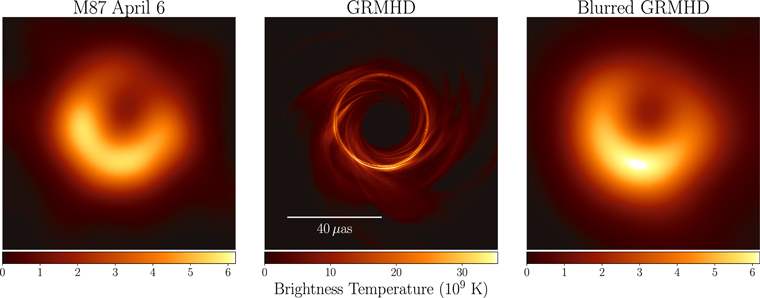
\includegraphics[width=\textwidth]{result-with-mhd.jpg}\\
%	\scriptsize\it(Left: Image from the Event Horizon Telescope. Center: Simulation of what it would look like. Right: 
%	The simulation, blurred to match the resolution of the EHT.)\EC
%}
%
%\frame{\frametitle{\textbf{Why this is a big deal}}
%	\BC
%	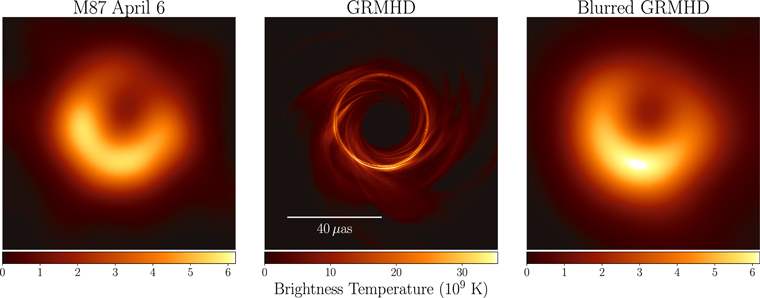
\includegraphics[width=\textwidth]{result-with-mhd.jpg}\\
%	\EC
%	
%	We've never seen a black hole before.
%	
%	\BS
%	
%	The light coming from the region near the event horizon is bent by the gravity of the black hole itself.
%	(This is why the central region is black.)
%	
%	\BS
%	
%	This gives us a picture of both the gas falling into a black hole, {\it and the gravity around a black hole}.
%	
%	\BS
%}
%
%




%       List of fallacies:
% done Ad hominem: violates objectivity
  % False ulterior motives
  % Actual ulterior motives
% done Argument from authority: the inverse of the preceding
% Sensationalism: violates objectivity and self-skepticism
% done Statistical shenanigans: violates empirical integrity
% done Cherry-picking: violates self-skepticism and/or empirical integrity
% done Ignoring refuting evidence: violates self-skepticism
% ``Island claims'': proposing something without considering the need to fit it into all the other things we know about our world
% Manufactured controversy: tobacco industry


%       Examples:
% EM-drive
% Moon landing hoax
% Water fluoridation hoax
% http://www.smokingaloud.com/
% GM corn in rats study
\end{document}
